\section{Harmonic maps for $F:S^k\ra S^k$}
\label{sec:harmonic-maps-skra}

\subsection{General properties}
\label{sec:general-properties}

From now on we shall set both the domain and target manifolds to
$S^k$. We choose the coordinates on the domain sphere as
\begin{align}
  \label{eq:9}
  x^a=(\psi,\theta),
\end{align}
where $\psi\in(0,\pi)$ is the longitudal angle with
south pole at $\psi=0$ and $\theta$ is the set of coordinates on
$S^{k-1}$ -- the equator of $S^k$. Analogously we introduce
coordinates $(\Psi,\Theta)$ on the target sphere in which the map $F$
takes the form
\begin{align}
  \label{eq:10}
  F^A(\psi,\theta)&=(\Psi,\Theta).
\end{align}
The metric tensors for the given coordinate frames are
\begin{align}
  \label{eq:11}
  &\text{domain:}&\quad &ds^2=d\psi^2+\sin^2\psi ds^2\big|_{S^{k-1}}\\
  &\text{target:}&\quad &dS^2=d\Psi^2+\sin^2\Psi dS^2\big|_{S^{k-1}}.
\end{align}
Solving equations \eqref{eq:8} without any further assumptions
presents an impossible task, we therefore in section
\ref{sec:basic-setup} introduce a simple ansatz. Still without any
simplifications we can state the following.

\begin{theorem}\label{thm:skk-energy-bound}
  For $k\ge3$ and any given map $F:S^k\ra S^k$ there is a map within
  the homotopy class of $F$ of arbitrary small Dirichlet energy.
\end{theorem}

\begin{proof}
  The proof is based on the fact that on a sphere there exists a one
  parameter group of conformal maps, which in the coordinates
  \eqref{eq:9} has the form
  \begin{align}
    \label{eq:12}
    \psi_A=2\arctan(e^A\tan(\psi/2)).
  \end{align}
  The above conformal map can be depicted as dragging the whole sphere
  along the longitudal coordinates in the direction of one of its
  poles (for $A$ large, this would be the north pole). We define the
  map $F_A$ to be the composition
  \begin{align}
    \label{eq:13}
    F_A=F\circ\psi_A.
  \end{align}
  As $\psi_A$ does leave the points $\psi=0$ and $\psi=\pi$ unchanged,
  $F_A$ has the same homotopy degree as $F$. Due to the conformal
  properties of the map $\psi_A$ we obtain the following energy
  density of $F_A$
  \begin{align}
    \label{eq:14}
    e(F_A)_\psi=&e(F)_{\psi_A}\rho_A^2,\\
    \rho_A=&\frac{1}{\cosh A-\cos\psi\sinh A},
  \end{align}
  where $e(F)_\psi$ is the energy density of $F$ at point $\psi$.  The
  map $F$ is regular, and therefore $e(F)_{\psi_A}$ is bounded by its
  maximal value $C(F)=\max_\psi\left(e(F)_\psi\right)$ therefore
  \begin{align}
    \label{eq:15}
    e(F_A)_\psi&\le C(F)\rho_A^2.
  \end{align}
  Assuming $k\ge3$, the Dirichlet energy of $F_A$ can be bounded by
  \begin{align}
    \label{eq:16}
    E(F_A)&=\int_{S^k}e(F_A)dV_{S^k}\\
    &\le C(F)V(S^{k-1})\int_{0}^{\pi}\rho_A^2\sin^{k-1}\psi d\psi\\
    &\le C(F)V(S^{k-1})\max_\psi(\sin^{k-3}\psi)\int_{0}^{\pi}\rho_A^2\sin^2\psi d\psi\\
    &\le C_1(F,k)\frac{1}{1+\cosh A}.
  \end{align}
  which can be made arbitrary small by an appropriate choice of
  $A$. The above bound is not optimal, but is sufficient for our
  purposes. As the map $\psi_A$ leaves the north and south poles of
  $S^k$ unchanged, the map $F_A$ is of the homotopy class that $F$ and
  we conclude by the following theorem.

\end{proof}



\subsection{Harmonic map ansatz}
\label{sec:basic-setup}

We simplify our problem by assuming that $\Theta=\theta$ and
$\Psi=f(\psi)$ so the map $F$ takes the form
\begin{align}
  \label{eq:17}
  F:(\psi,\theta)\ra(f(\psi),\theta),
\end{align}
which leaves us with one function as a degree of freedom. The given
setup has been introduced in ~\cite{Eells1964} and it consists of the
idea that, after removing the poles, $S^k$ can be treated as
$(0,\pi)\times S^{k-1}$, for which we can use remarks \ref{rem:1} and
\ref{rem:2} with $F_1=f$ and $F_2=\id$.\\

For $F$ to be continuous, we require that
\begin{align}
  \label{eq:18}
  \lim_{\psi\ra0}f(\psi)=n\pi,\quad\lim_{\psi\ra\pi}f(\psi)=m\pi.
\end{align}
Moreover, closing the domain of $\psi$ will not have any implications
as long as $F$ is regular so we can drop the limits from \eqref{eq:18}
\begin{align}
  \label{eq:19}
  f(0)=n\pi\quad f(\pi)=m\pi.
\end{align}
The number $n-m$ stands for the homotopy degree of a
map.\\

The Dirichlet energy of the considered map has now a more transparent
form
\begin{align}
  \label{eq:20}
  E(f)=\frac{1}{2}\int_{0}^{\pi}
  \left(f'^2+(k-1)\frac{\sin^2f}{\sin^2\psi}\right) \sin^{k-1}\psi
  d\psi,
\end{align}
where we have changed the argument of $E$ from $F$ to $f$ as
effectively it is a functional of $f$ and we have dropped the volume
term $V(S^{k-1})$ which has no qualitative impact on the behaviour of
the system.
% The energy density of \eqref{eq:20} with the volume
% term $V(S^{k-1})$ dropped is
% \begin{align}
%   \label{eq:21}
%   e(f)=\frac{1}{2}\left(f'^2+(k-1)\frac{\sin^2f}{\sin^2\psi}\right).
% \end{align}
By the definition \ref{def:regular-map}, the map $f$ is regular if
\begin{align}
  \label{eq:22}
  e(f)=\frac{1}{2}\left(f'^2+(k-1)\frac{\sin^2f}{\sin^2\psi}\right)<\infty.
\end{align}
% The Dirichlet energy of $f$ is
% \eqref{eq:20}
% \begin{align}
%   \label{eq:23}
%   E(f)=\int_0^\pi e(f)\sin^{k-1}\psi d\psi\ge0.
% \end{align}

Critical points of $E(f)$ are solutions to the corresponding
Euler-Lagrange equation
\begin{align}
  \label{eq:f_psi_EL} \frac{1}{\sin^{k-1}\psi}\left(\sin^{k-1}\psi
    f'\right)'-\frac{(k-1)}{2}\frac{\sin2f}{\sin^2\psi}=0.
\end{align} with the boundary values
\begin{align}
  \label{eq:24} f(0)=n\pi,\quad f(\pi)=m\pi.
\end{align} The equation \eqref{eq:f_psi_EL} has trivial solutions
$f=n\pi$ of homotopy degree zero for which $E(f)$ attains absolute
minimum: $E(n\pi)=0$. By remark \ref{rem:1}, the identity map
$f=\psi+n\pi$ is also the solution but of the homotopy degree one.
Hereafter we set $n=0$ without loss of generality.
% Because in general, the symmetry
% \begin{align}
%   \label{eq:25}
%   E(f+n\pi)=E(f)
% \end{align} implies that any stationary point of $E$ remains
% stationary after being translated by $n\pi$ we henceforth drop the
% inessential ``$+n\pi$'' to simplify the notion of possible
% solutions.
By the nontrivial $\mathbb{Z}_2$ symmetry (the antipodal
reflection)
\begin{align}
  \label{eq:26}
  f&\ra \bar{f}=\pi-f,\\
  E(f)&\ra E(\bar{f})=E(f),
\end{align}
every possible critical point will have its partner of the same
homotopy degree. This is true unless $f$ is invariant under
\eqref{eq:26}, but the only such case is $f_e=\pi/2$ which is not
continuous thus not harmonic. (TODO: it does however play an important
role and is described in grater detail in appendix). To be consistent
with \cite{Bizon1997} we shall denote the constant and identity
solutions as
\begin{align}
  \label{eq:27}
  f_0=0\quad f_1=\psi.
\end{align}
These, are the only solutions to \eqref{eq:f_psi_EL} known in the
closed form. More detailed analysis of \eqref{eq:f_psi_EL} is
contained in \cite{Bizon1997} and \cite{Corlette2001}, where the
infinite family of regular solutions for $3\le k\le6$ has been
found. Following the notation in \cite{Bizon1997}, we denote the
solutions as $f_n$, where $n\in\mathbb{N}_0$. The parametrization by
$n$ is motivated by the property that $f_n$ has exactly $n$
intersections with $\pi/2$ and $n-1$ extrema. Each of $f_n$ is of
homotopy degree zero for $n$ even or one for $n$ odd and stays inside
the square $[0,\pi]\times[0,\pi]$. To be consistent with \eqref{eq:27}
we set $f_n(0)=0$. The first few such harmonic maps are depicted in
figure \ref{fig:Harmonic_maps}. From \cite{Bizon1997} it also follows
that the solutions obey the following parity relation
\begin{align}
  \label{eq:28}
  f_n(\psi)=(-1)^n f_n(\pi-\psi).
\end{align}

\begin{figure}[ht]
  \centering
  \label{fig:Harmonic_maps}
  % GNUPLOT: LaTeX picture with Postscript
\begingroup
  \makeatletter
  \providecommand\color[2][]{%
    \GenericError{(gnuplot) \space\space\space\@spaces}{%
      Package color not loaded in conjunction with
      terminal option `colourtext'%
    }{See the gnuplot documentation for explanation.%
    }{Either use 'blacktext' in gnuplot or load the package
      color.sty in LaTeX.}%
    \renewcommand\color[2][]{}%
  }%
  \providecommand\includegraphics[2][]{%
    \GenericError{(gnuplot) \space\space\space\@spaces}{%
      Package graphicx or graphics not loaded%
    }{See the gnuplot documentation for explanation.%
    }{The gnuplot epslatex terminal needs graphicx.sty or graphics.sty.}%
    \renewcommand\includegraphics[2][]{}%
  }%
  \providecommand\rotatebox[2]{#2}%
  \@ifundefined{ifGPcolor}{%
    \newif\ifGPcolor
    \GPcolorfalse
  }{}%
  \@ifundefined{ifGPblacktext}{%
    \newif\ifGPblacktext
    \GPblacktexttrue
  }{}%
  % define a \g@addto@macro without @ in the name:
  \let\gplgaddtomacro\g@addto@macro
  % define empty templates for all commands taking text:
  \gdef\gplbacktext{}%
  \gdef\gplfronttext{}%
  \makeatother
  \ifGPblacktext
    % no textcolor at all
    \def\colorrgb#1{}%
    \def\colorgray#1{}%
  \else
    % gray or color?
    \ifGPcolor
      \def\colorrgb#1{\color[rgb]{#1}}%
      \def\colorgray#1{\color[gray]{#1}}%
      \expandafter\def\csname LTw\endcsname{\color{white}}%
      \expandafter\def\csname LTb\endcsname{\color{black}}%
      \expandafter\def\csname LTa\endcsname{\color{black}}%
      \expandafter\def\csname LT0\endcsname{\color[rgb]{1,0,0}}%
      \expandafter\def\csname LT1\endcsname{\color[rgb]{0,1,0}}%
      \expandafter\def\csname LT2\endcsname{\color[rgb]{0,0,1}}%
      \expandafter\def\csname LT3\endcsname{\color[rgb]{1,0,1}}%
      \expandafter\def\csname LT4\endcsname{\color[rgb]{0,1,1}}%
      \expandafter\def\csname LT5\endcsname{\color[rgb]{1,1,0}}%
      \expandafter\def\csname LT6\endcsname{\color[rgb]{0,0,0}}%
      \expandafter\def\csname LT7\endcsname{\color[rgb]{1,0.3,0}}%
      \expandafter\def\csname LT8\endcsname{\color[rgb]{0.5,0.5,0.5}}%
    \else
      % gray
      \def\colorrgb#1{\color{black}}%
      \def\colorgray#1{\color[gray]{#1}}%
      \expandafter\def\csname LTw\endcsname{\color{white}}%
      \expandafter\def\csname LTb\endcsname{\color{black}}%
      \expandafter\def\csname LTa\endcsname{\color{black}}%
      \expandafter\def\csname LT0\endcsname{\color{black}}%
      \expandafter\def\csname LT1\endcsname{\color{black}}%
      \expandafter\def\csname LT2\endcsname{\color{black}}%
      \expandafter\def\csname LT3\endcsname{\color{black}}%
      \expandafter\def\csname LT4\endcsname{\color{black}}%
      \expandafter\def\csname LT5\endcsname{\color{black}}%
      \expandafter\def\csname LT6\endcsname{\color{black}}%
      \expandafter\def\csname LT7\endcsname{\color{black}}%
      \expandafter\def\csname LT8\endcsname{\color{black}}%
    \fi
  \fi
  \setlength{\unitlength}{0.0500bp}%
  \begin{picture}(7200.00,5040.00)%
      \csname LTb\endcsname%
      \put(3600,4820){\makebox(0,0){\strut{}Harmonic maps between spheres}}%
    \gplgaddtomacro\gplbacktext{%
    }%
    \gplgaddtomacro\gplfronttext{%
    }%
    \gplgaddtomacro\gplbacktext{%
      \csname LTb\endcsname%
      \put(2160,4328){\makebox(0,0){\strut{}$f_1$}}%
    }%
    \gplgaddtomacro\gplfronttext{%
    }%
    \gplgaddtomacro\gplbacktext{%
    }%
    \gplgaddtomacro\gplfronttext{%
    }%
    \gplgaddtomacro\gplbacktext{%
      \csname LTb\endcsname%
      \put(5040,4328){\makebox(0,0){\strut{}$f_2$}}%
    }%
    \gplgaddtomacro\gplfronttext{%
    }%
    \gplgaddtomacro\gplbacktext{%
    }%
    \gplgaddtomacro\gplfronttext{%
    }%
    \gplgaddtomacro\gplbacktext{%
      \csname LTb\endcsname%
      \put(2160,2984){\makebox(0,0){\strut{}$f_3$}}%
    }%
    \gplgaddtomacro\gplfronttext{%
    }%
    \gplgaddtomacro\gplbacktext{%
    }%
    \gplgaddtomacro\gplfronttext{%
    }%
    \gplgaddtomacro\gplbacktext{%
      \csname LTb\endcsname%
      \put(5040,2984){\makebox(0,0){\strut{}$f_4$}}%
    }%
    \gplgaddtomacro\gplfronttext{%
    }%
    \gplgaddtomacro\gplbacktext{%
      \csname LTb\endcsname%
      \put(588,504){\makebox(0,0)[r]{\strut{}0}}%
      \put(588,1176){\makebox(0,0)[r]{\strut{}$\pi/2$}}%
      \put(588,1847){\makebox(0,0)[r]{\strut{}$\pi$}}%
      \put(588,504){\makebox(0,0)[r]{\strut{}}}%
      \put(588,840){\makebox(0,0)[r]{\strut{}}}%
      \put(588,1176){\makebox(0,0)[r]{\strut{}}}%
      \put(588,1511){\makebox(0,0)[r]{\strut{}}}%
      \put(588,1847){\makebox(0,0)[r]{\strut{}}}%
      \put(720,284){\makebox(0,0){\strut{}-10}}%
      \put(1440,284){\makebox(0,0){\strut{}-5}}%
      \put(2160,284){\makebox(0,0){\strut{} 0}}%
      \put(2880,284){\makebox(0,0){\strut{} 5}}%
      \put(3600,284){\makebox(0,0){\strut{} 10}}%
      \put(-3,1175){\rotatebox{90}{\makebox(0,0){\strut{}$f_n(\psi)$}}}%
      \put(2160,89){\makebox(0,0){\strut{}$\ln(\tan(\psi/2))$}}%
    }%
    \gplgaddtomacro\gplfronttext{%
    }%
    \gplgaddtomacro\gplbacktext{%
      \csname LTb\endcsname%
      \put(588,504){\makebox(0,0)[r]{\strut{}0}}%
      \put(588,1176){\makebox(0,0)[r]{\strut{}$\pi/2$}}%
      \put(588,1847){\makebox(0,0)[r]{\strut{}$\pi$}}%
      \put(588,504){\makebox(0,0)[r]{\strut{}}}%
      \put(588,840){\makebox(0,0)[r]{\strut{}}}%
      \put(588,1176){\makebox(0,0)[r]{\strut{}}}%
      \put(588,1511){\makebox(0,0)[r]{\strut{}}}%
      \put(588,1847){\makebox(0,0)[r]{\strut{}}}%
      \put(720,284){\makebox(0,0){\strut{}-10}}%
      \put(1440,284){\makebox(0,0){\strut{}-5}}%
      \put(2160,284){\makebox(0,0){\strut{} 0}}%
      \put(2880,284){\makebox(0,0){\strut{} 5}}%
      \put(3600,284){\makebox(0,0){\strut{} 10}}%
      \put(-3,1175){\rotatebox{90}{\makebox(0,0){\strut{}$f_n(\psi)$}}}%
      \put(2160,89){\makebox(0,0){\strut{}$\ln(\tan(\psi/2))$}}%
      \put(2160,1640){\makebox(0,0){\strut{}$f_5$}}%
    }%
    \gplgaddtomacro\gplfronttext{%
    }%
    \gplgaddtomacro\gplbacktext{%
    }%
    \gplgaddtomacro\gplfronttext{%
    }%
    \gplgaddtomacro\gplbacktext{%
      \csname LTb\endcsname%
      \put(5040,1640){\makebox(0,0){\strut{}$f_6$}}%
    }%
    \gplgaddtomacro\gplfronttext{%
    }%
    \gplbacktext
    \put(0,0){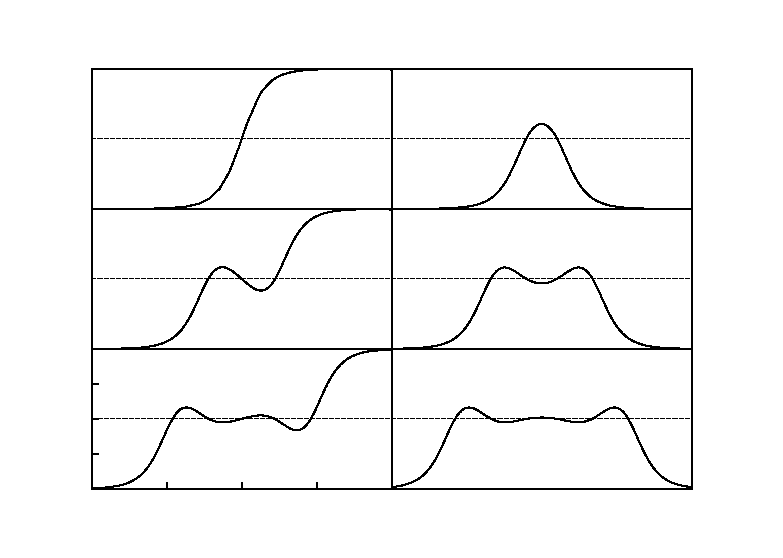
\includegraphics{graphics/Harmonic_static_to_multiplot}}%
    \gplfronttext
  \end{picture}%
\endgroup

  \caption{The first six non-trivial solutions to \eqref{eq:f_psi_EL}}
\end{figure}

In \cite{Corlette2001} the authors proved that $f_n$ has index $n$
(there are $n$ negative eigenvalues of the Hessian of the
energy). From the last statement it follows that there are no local
minima of $E(f)$ apart from $f_0$. As we will need the following
property later on we introduce it in a form of the theorem
\begin{theorem}[Wald,Corlette]
  \label{thm:harmonic-map-index}
  There are no local minima of $E(f)$ apart from $f=n\pi$.
\end{theorem}
\begin{proof}
  This can also be proved by showing that for each $n>0$, $f_n$ there
  is at least one direction $v$ for which the Hessian is negative
  \begin{align}\label{eq:29}
    \delta^2E(f_n)(v,v) &=\int_0^{\pi} \left(
      v'^2+(k-1)\frac{\cos2f_n}{\sin^2\psi}v^2 \right)\sin^{k-1}\psi
    d\psi\\
    &=(v,\mathcal{L}_n v),\\
    \mathcal{L}_nv&=-\frac{1}{\sin^{k-1}\psi}\left(\sin^{k-1}\psi
      v'\right)'+(k-1)\frac{\cos2f_n}{\sin^2\psi}v
  \end{align}
  It turns out that the conformal Killing on $S^k$
  field
  \begin{align}
    \label{eq:30}
    K=\sin\psi\frac{\partial}{\partial\psi}
  \end{align}
  related to \eqref{eq:12} generates such $v$, namely for $v=\sin\psi
  f_n'(\psi)$ by \eqref{eq:strange_variation} we have
  \begin{align}
    \label{eq:31}
    \mathcal{L}_n v&=(2-k)v\\
    \delta^2 E(f_n)(v,v)&=(v,\mathcal{L}_n v)=(2-k)\lVert v\rVert^2<0.
  \end{align}
  This construction does not hold for $n=0$ in which case $v$ is the
  null direction.
\end{proof}

%%% Local Variables:
%%% mode: latex
%%% TeX-master: "master"
%%% End:
